\documentclass[a4paper,12pt]{article}
% \input{../../../config.tex}
\usepackage{mypackages}
\usepackage{macros}


\titleformat{\section}
  {\color{red}\normalfont\Large\bfseries}
  {\thesection}{1em}{}

\titleformat{\subsection}
  {\color{blue}\normalfont\large\bfseries}
  {\thesubsection}{1em}{}

\titleformat{\subsubsection}
  {\color{magenta}\normalfont\normalsize\bfseries}
  {\thesubsubsection}{1em}{}

\setlength{\parindent}{0pt}

\begin{document}

\title{Réunion parents professeurs}
\author{N. Bancel}
\date{Septembre 2024}
\maketitle

\section{Section internationale}

\subsection*{Physique - Chimie}

\subsubsection*{Présentation rapide}

\subsubsection*{Objectifs de l'année}

\textcolor{brown}{\textbf{Compétences}}

\begin{itemize}[noitemsep]
\item Pratique de démarches scientifiques (questions, hypothèses, interpréter)
\item Concevoir, réaliser un dispositif de mesure et d'observation
\item S'approprier des outils et des méthodes (recherches bibliographiques, utiliser des outils numériques)
\item Expression écrite et orale 
\item Adapter un comportement éthique et responsable (sécurité en physique / chimie, réinvestir ses connaissances)
\item Se situer dans l'espace et dans le temps
\end{itemize}

\textcolor{brown}{\textbf{Echéances}}

\begin{itemize}[noitemsep]
  \item Brevet en Juillet
  \item Préparation au programme et aux méthodes attendues au lycée
\end{itemize}


\subsubsection*{Méthodes pédagogiques}


\begin{itemize}[noitemsep]
  \item Alternance entre 2 types de format :
    \begin{itemize}[noitemsep]
      \item Notes prises en recopiant le tableau. Importance de prendre en main, structurer des raisonnements scientifiques : 
      \begin{itemize}[noitemsep]
        \item Enoncé / reformulation du problème
        \item Section théorique (formule + définition des variables)
        \item Application numérique (lister les données, convertir, remplacer dans la formule, fournir le résultat final)
        \item Interpréter le résultat
      \end{itemize}
      \item Ecriture sur un polycopié pré rempli.
    \end{itemize}
  \item Apprentissage par la mise en pratique
    \begin{itemize}[noitemsep]
      \item Nombreux exercices faits pendant le cours
      \item 1 projet par chapitre. Souvent volontairement large, peu guidé.
        \begin{itemize}[noitemsep]
          \item En lien avec la maison (Chimie, Electricité, Energie : tout est à disposition)
          \item Travail sur la capacité à conceptualiser
          \item Jouer le jeu de ne pas trop aider sur ces projets, ni utiliser ChatGPT
        \end{itemize}
    \end{itemize}
  \end{itemize}
  

\subsubsection*{Routine + Evaluations}

\begin{itemize}[noitemsep]
  \item Petit test (30 minutes) noté à chaque fin de chapitre (évaluation des compétences)
  \item 1 à 2 devoirs surveillés par trimestre (2h)
  \item Exercices à faire chez soi et corrigés en cours
  \item 1 projet peu guidé par chapitre - non noté, corrigé mis en ligne sur EcoleDirecte 
\end{itemize}

\subsubsection*{Rôle des parents} 

\begin{itemize}[noitemsep]
  \item Vérification que devoirs faits. Ne pas trop aider sur la réalisation des devoirs
  \item Communication ouverte : Disponible pour discuter de progrès de l'élève 
\end{itemize}


\subsection*{Projets scientifiques}


\subsubsection*{Commun à toutes les classes - Utilisation de l'imprimante 3D}

\begin{itemize}[noitemsep]
  \item Travail sur OnShape - logiciel de modeling 3D. Permet de travailler la géométrie dans l'espace, comprendre des spécifications, en créer. Industriel + permet de prototyper
  \item Impressions 3D de petits objets au choix
  \item Utilisation plus généralisée à des projets autres que les projets scientifiques
\end{itemize}

\begin{figure}[H]
  \centering
  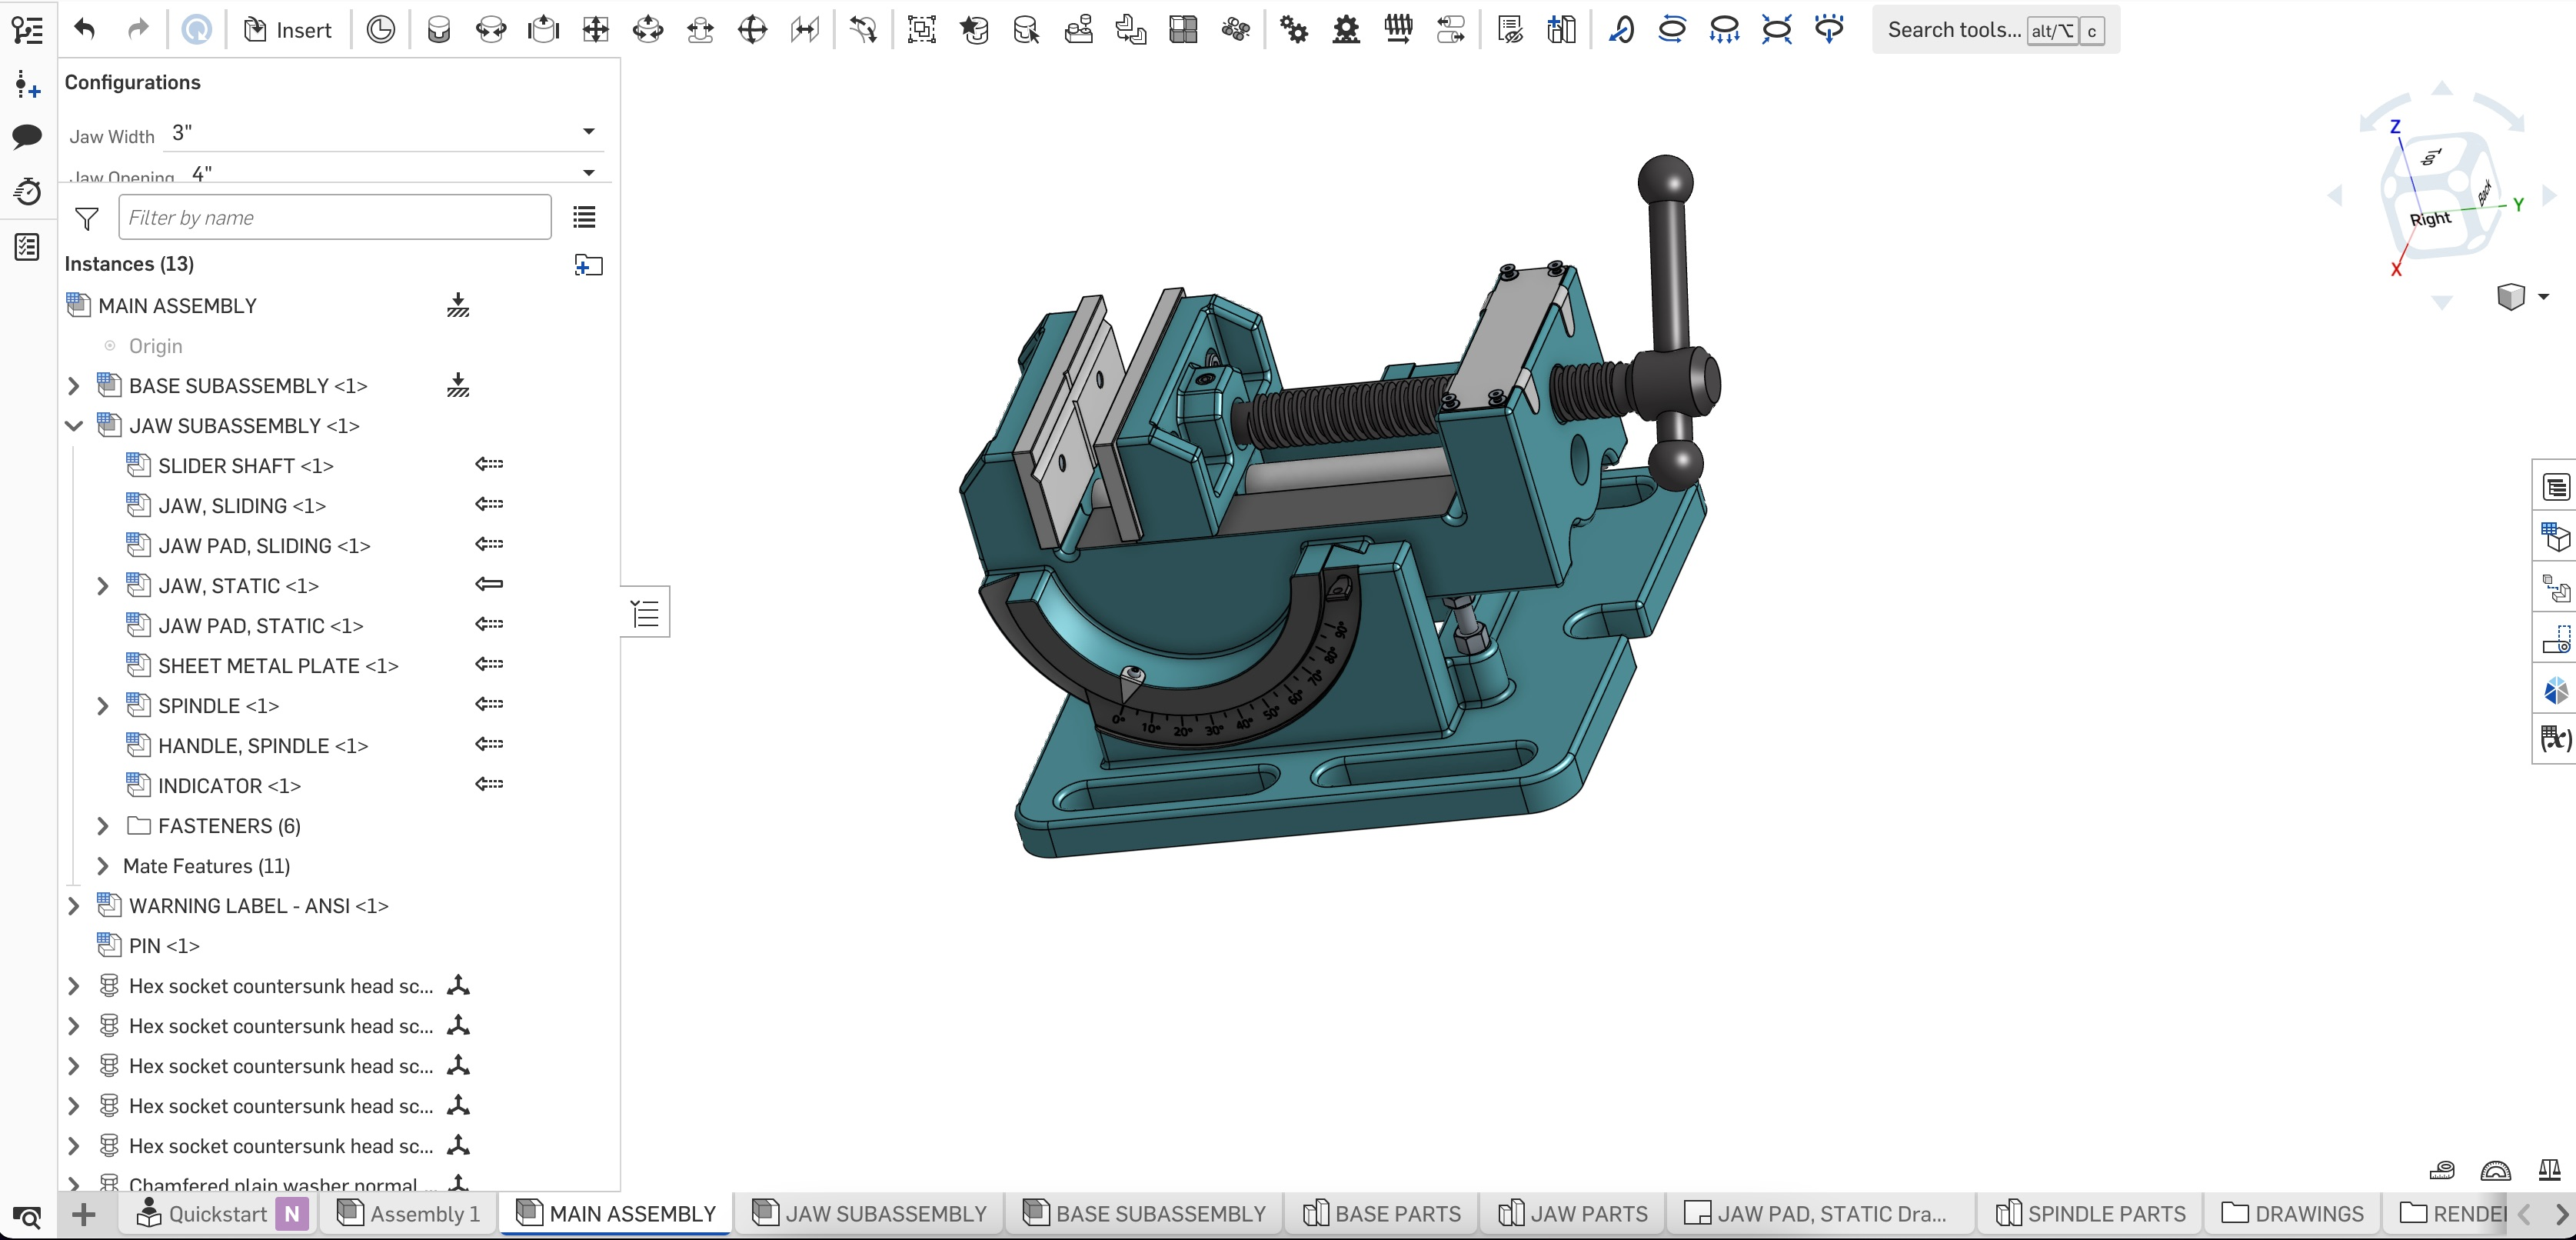
\includegraphics[width=\linewidth]{onshape.jpg}
  \caption{\label{} Logiciel OnShape}
\end{figure}

\subsubsection*{Projet 4ème / 3ème - Lombricomposteur}

\begin{itemize}[noitemsep]
  \item Principe : compost digéré par des verres qui produisent de l'engrais naturel (lombricompost) et de l'engrais liquide organique. 
  \item Construction
  \begin{itemize}[noitemsep]
    \item Etages en bois 
    \item Robinet + récupérateur de jus
    \item Roulettes
  \end{itemize}
  \item Prototypage avec imprimante 3D
  \item Potentiel projet additionnel : potager à Suger. Pour utiliser l'engrais
\end{itemize}


\begin{figure}[H]
  \centering
  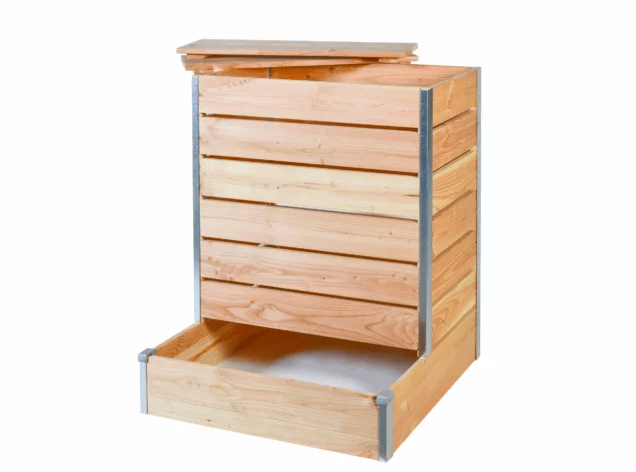
\includegraphics[width=0.5\linewidth]{lombri_png.png}
  \caption{\label{} Lombricomposteur}
\end{figure}

\subsubsection*{Projet 6ème / 5ème - Un ballon dans l'espace}

\begin{itemize}[noitemsep]
  \item Ballon à l'hélium envoyé dans l'espace 
  \item Lien : \href{https://www.planete-sciences.org/espace/Ballon-stratospherique/Un-ballon-pour-l-ecole?lang=fr}{Un ballon pour l'école}
  \item Echeances : 
    \begin{itemize}[noitemsep]
      \item jusqu’au 29 septembre : dépôt des dossiers de candidature
      \item jeudi 10 octobre : sélection des dossiers
      \item octobre et février : formations Planète Sciences
      \item octobre à avril : 3 visites de l’animateur « suiveur » de Planète Sciences dans la classe ou à distance
      \item avril à juin : lâchers de ballons réalisés par nos aérotechniciens
      \item juin à septembre : transmission du compte-rendu réalisé par la classe et renvoi des émetteurs
    \end{itemize}
  \item Prototypage de la nacelle - Photos / GoPro dans la nacelle
  \end{itemize}

  \begin{figure}[H]
    \centering
    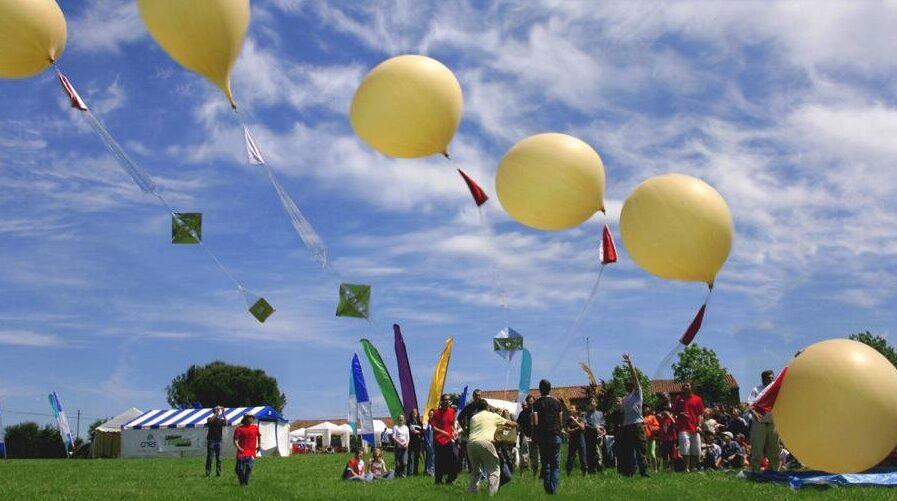
\includegraphics[width=0.7\linewidth]{ballon.jpg}
    \caption{\label{} Un ballon pour l'école}
  \end{figure}

\end{document}

